\section{Pruebas del sistema}
\label{sec:Pruebas del sistema}
    En esta secci\'on se describen y documentan las diferentes pruebas realizadas al sistema desarrollado. 
        Estas pruebas se realizaron con el objetivo de verificar el correcto funcionamiento del sistema y 
        de identificar posibles errores o fallas en el c\'odigo. Las pruebas se realizaron en diferentes 
        etapas del desarrollo del sistema, desde la implementaci\'on de los m\'odulos hasta la integraci\'on 
        de los mismos. Primero para cada uno de los productos desarrollados, el simulador del Physarum
        Polycephalum y el sistema de monitoreo poblacional, se describen como son las pruebas que se realizaron
        y los resultados obtenidos. Posteriormente se describen las pruebas correspondientes para cada uno de los productos.
    \subsection{An\'alisis de primera iteraci\'on de datos de sensores } % (fold)
    En esta primera iteraci\'on, se recopilaron y analizaron los datos de los sensores 
        integrados en el sistema, con el objetivo de comprender el tipo de informaci\'on 
        proporcionada por el LiDAR y las c\'amaras utilizadas, as\'i como su potencial para la 
        implementaci\'on de una interfaz gr\'afica. Esta fase fue crucial, ya que marc\'o el punto 
        de partida para la integraci\'on de los datos sensoriales en un entorno visual que permitiera 
        la interpretaci\'on y el control en tiempo real.
    \vskip 0.5cm
    El sensor LiDAR proporcion\'o datos en formato de coordenadas cartesianas, calculadas a 
        partir de distancias y \'angulos. Estos datos permiten la representaci\'on de un mapa 
        del entorno en dos dimensiones, detectando la proximidad de objetos y obst\'aculos 
        en el \'area circundante. La informaci\'on recopilada incluy\'o principalmente mediciones 
        de distancia en mil\'imetros, asociadas a coordenadas angulares espec\'ificas, las cuales 
        se convirtieron en valores cartesianas para su futura visualizaci\'on en una interfaz gr\'afica. 
        Por ejemplo, las primeras mediciones capturadas del LiDAR ofrec\'ian distancias que oscilaban 
        entre los 20 cm y los 5 metros, brindando una imagen b\'asica del espacio inmediato.
    \vskip 0.5cm
    Por otro lado, se evaluaron diferentes tipos de c\'amaras, las cuales proporcionaban datos en diversos 
        formatos. Se analizaron c\'amaras que ofrec\'ian salidas en formatos como Modelo de color YUV 
        (no tiene un significado literal en t\'erminos de siglas, pero com\'unmente se describe por sus componentes: 
        Y para luminancia, y U y V para crominancia), incluyendo variantes (YUV420, YUV422) y 
        RGB, siendo el formato YUV uno de los m\'as eficientes para transmisi\'on y procesamiento de video, 
        especialmente en aplicaciones que requieren una compresi\'on de alta calidad. Este formato divide la 
        informaci\'on de luminancia (Y) y crominancia (UV), lo que facilita la reducci\'on del ancho de banda 
        necesario sin comprometer la calidad visual en exceso. Durante las pruebas iniciales, el formato YUV422 
        mostr\'o ser particularmente adecuado para entornos donde la transmisi\'on r\'apida de im\'agenes era prioritaria, 
        dado que proporcionaba una mayor eficiencia en t\'erminos de compresi\'on de datos en comparaci\'on con RGB, 
        aunque con menos fidelidad en los detalles de color.
    \vskip 0.5cm
    La c\'amara RGB tambi\'en fue evaluada para obtener im\'agenes con una representaci\'on precisa de los colores del 
        entorno. A diferencia del formato YUV, los datos RGB capturan la totalidad de la informaci\'on de color, 
        lo que result\'o \'util en situaciones donde se requer\'ia una mayor claridad visual para la identificaci\'on 
        de objetos. Sin embargo, el formato RGB mostr\'o ser menos eficiente en t\'erminos de tama\~no de archivo y 
        procesamiento, lo que lo hac\'ia menos adecuado para aplicaciones en tiempo real donde la optimizaci\'on 
        del rendimiento era cr\'itica.
    \vskip 0.5cm
    El an\'alisis de esta primera iteraci\'on fue fundamental para comprender las capacidades y limitaciones de los 
        sensores, lo que permiti\'o decidir sobre los formatos de datos m\'as adecuados para su futura implementaci\'on 
        en una interfaz gr\'afica. Se identific\'o que los datos del LiDAR ofrec\'ian una representaci\'on clara y precisa 

        del entorno inmediato, mientras que las diferentes c\'amaras evaluadas proporcionaban flexibilidad en la 
        captura de informaci\'on visual, dependiendo de los requisitos de resoluci\'on y velocidad de procesamiento.
% subsection An\'alisis de Primera Iteraci\'on de Datos de Sensores  (end)
    \subsection{Diseño de módulos de hardware del robot para pruebas de integración}
    %Parrafo 1
    En esta sección se detalla el diseño de los módulos de hardware del robot que hemos
        desarrollado para el Trabajo Terminal. El objetivo principal es asegurar una integración
        eficiente entre los diferentes componentes, permitiendo así la realización de pruebas
        de integración efectivas. La modularidad del diseño facilita tanto el desarrollo como el
        mantenimiento del sistema, así como también la sustitución de algunos componentes,
        esto nos permite aislar y solucionar problemas de manera aislada.
    \vskip 0.5cm
    %Parrafo 2
    Nuestro robot desarrollado consta de cuatro módulos principales: actuadores,
        sensores, unidad de control y módulo de visualización. Cada uno de estos módulos
        cumple una función especifica que permite al robot moverse, detectar obstáculos, y
        seguir rutas predefinidas.
    \vskip 0.5cm
    %Figura 1
    \begin{figure}[htbp]
        \centering
        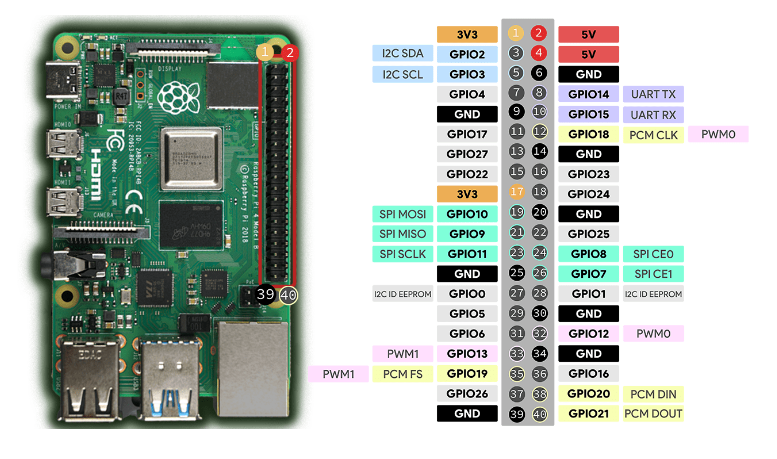
\includegraphics[width=0.5\textwidth]{./images/Pruebas/robot/robot01.png}
        \caption{Diseño de los pines de configuracion de los módulos de hardware del robot.}
        \label{fig:robot}
    \end{figure}

    \subsubsection{M\'odulo de actuadores (Motores)} % (fold)
    \label{ssub:modact}
    El robot está equipado por cuatro motores a pasos Nema 23, controlados a través de
        un controlador driver específico para motores a pasos. Estos motores son
        responsables del movimiento del robot en las direcciones deseadas, permitiendo giros,
        avances y retrocesos mediante la manipulación precisa de los pines de control PWM y
        de dirección.
    \vskip 0.5cm
    Los motores Nema 23 fueron elegidos debido a su precisión en el posicionamiento y
        su capacidad para generar el torque necesario para mover la estructura del robot, que
        está construida con perfiles de aluminio y ruedas omnidireccionales.
    \vskip 0.5cm
    % tabla 1
    \begin{longtable}{|c|c|c|c|}
        \hline
        \rowcolor{gray}
        \textbf{Producto} & \textbf{Descripci\'on} & \textbf{Piezas} \\
        \hline
        Motor a pasos Nema 23 & Motor a pasos Nema 23 con placa frontal & 4  \\
        Controlador de motores a pasos & Controlador de motores a pasos TB6600 & 4  \\
        Rueda omnidireccional & Rueda omnidireccional de 6 in & 4  \\
        \hline
        \caption{Especificaciones de los motores a pasos Nema 23.}
        \label{tab:motor}
    \end{longtable}
    \vskip 0.5cm
    Los motores están conectados a los pines GPIO de la Raspberry Pi 4 B mediante un
        controlador de moteres. El sistema de control utiliza señales PWM para regular la
        velocidad de los motores, y señales de dirección para controlar el sentido de giro.
    \vskip 0.5cm
    Elegimos los Motores Nema 23 debido a su precisión y capacidad de generar torque
        necesario para mover el robot con su estructura de aluminio y ruedas
        omnidireccionales. Su tamaño y especificaciones son ideales para aplicaciones que
        requieren alta precisión en el movimiento.
    \vskip 0.5cm
    La incorporación de ruedas omnidireccionales de 6 pulgadas permite al robot realizar
        movimientos en varias direcciones sin necesidad de girar su estructura por completo.
        Esto optimiza la maniobrabilidad en entornos reducidos
    \vskip 0.5cm
    Finalmente elegimos los controladores a pasos por que estos son capaces de manejar
        la corriente y el voltaje necesario para los motores Nema 23, permitiendo un control
        preciso mediante señales PWM generadas desde la unidad de control.}
    \vskip 0.5cm
    % subsubsection  (end)
    \subsubsection{M\'odulo de sensores} % (fold)
    \label{ssub:modsen}
    El robot está equipado por un sensor YLiDAR 2XL, que permite realizar un escaneo de
    360° del entorno para detectar obstáculos y mapear el área de operación del robot. La
    elección de este sensor se debe a su capacidad para medir distancias con alta
    precisión y su adecuado rango de operación, lo que lo convierte en una opción ideal
    para la navegación autónoma en tiempo real.
    El sensor se conecta a la unidad de control mediante un puerto USB tipo A.
    % subsubsection  (end)
    \subsection{Desarrollo de m\'odulos de hardware del robot para pruebas de integraci\'on}
\label{sec:Desarrollo de m\'odulos de hardware del robot para pruebas de integraci\'on}
    % Parrafo 1
    En la siguiente secci\'on vamos a detallar el proceso de implementaci\'on de los m\'odulos
        de hardware que componen el robot. Se describir\'an las decisiones t\'ecnicas tomadas
        durante la construcci\'on, la integraci\'on f\'isica y funcional de los m\'odulos, y los
        resultados preliminares de las pruebas iniciales. El objetivo es mostrar c\'omo los
        m\'odulos de actuadores, sensores, la unidad de control y sistema de visualizaci\'on
        fueron desarrollados para llevar a cabo las pruebas de integraci\'on.
    \vskip 0.5cm
    \subsubsection{M\'odulo de actuadores}
    El m\'odulo de actuadores est\'a compuesto por cuatro motores Nema 23 conectados a
        ruedas omnidireccionales. Los motores se montaron sobre una base de perfiles de
        aluminio 2040, elegidos por su resistencia y ligereza. Los motores se conectaron a susrespectivos controladores mediante cables blindados para reducir interferencias
        electromagn\'eticas.
    \vskip 0.5cm
    Para el control de los motores, se utiliz\'o la Raspberry Pi, que env\'ia se\~nales PWM a
        trav\'es de sus pines GPIO, controlando la velocidad y direcci\'on de los motores. Se
        ajust\'o la frecuencia de las se\~nales PWM a 400 Hz, lo que permiti\'o un control suave y
        preciso del movimiento del robot.
    \vskip 0.5cm
    Para poder controlar los motores, se desarroll\'o un c\'odigo en C++ que utiliz\'o la
        biblioteca pigpio para gestionar las se\~nales PWM. El c\'odigo permite ajustar tanto la
        velocidad como la direcci\'on de los motores en tiempo real.
    \vskip 0.5cm
    \begin{lstlisting}[language={C++}, caption={C\'odigo de ejemplo de motores}, label={Script}]
        void setMotorSpeed(int motor, int frequency) {
            if (motor >= 0 && motor < 4) {
                gpioSetPWMfrequency(PWM_PINS[motor], frequency);
            }
        }
        void setMotorDirection(int motor, int direction) {
            if (motor >= 0 && motor < 4) {
                gpioWrite(DIR_PINS[motor], direction);
            }
        }
    \end{lstlisting}
    \vskip 0.5cm
    \subsubsection{M\'odulo de sensores}
    El sensor LiDAR YDLIDAR 2XL fue montado en la parte superior del robot para obtener
        un \'angulo de escaneo de 360 grados. El sensor se conect\'o a la Raspberry Pi a trav\'es de
        un puerto USB A. La configuraci\'on f\'isica permiti\'o que el LiDAR tuviera una vista
        despejada del entorno, crucial para la detecci\'on precisa de obst\'aculos.
    \vskip 0.5cm
    El sensor LiDAR se configur\'o utilizando la biblioteca proporcionada por el fabricante
        (YLiDAR SDK) y se desarroll\'o un c\'odigo para la lectura continua de los datos de escaneo.
        Los datos obtenidos del LiDAR se procesaron en tiempo real para permitir la
        navegaci\'on aut\'onoma y la detecci\'on de obst\'aculos.
    \vskip 0.5cm
    \begin{lstlisting}[language={C++}, caption={Primero se implementa la librer\'ia del LiDAR}, label={Script}]
        #include "CYdLidar.h"
        using namespace ydlidar;
    \end{lstlisting}
    \vskip 0.5cm
    Despu\'es se inicializa el sensor y se obtienen los datos de escaneo:
    \vskip 0.5cm
    \begin{lstlisting}[language={C++}, caption={Configuraci\'on de opciones del LiDAR}, label={Script}]
        CYdLidar laser;
        laser.setlidaropt(LidarPropSerialPort, port.c_str(), port.size());
        std::string ignore_array;
        ignore_array.clear();
        laser.setlidaropt(LidarPropIgnoreArray, ignore_array.c_str(), ignore_array.size());

        laser.setlidaropt(LidarPropSerialBaudrate, &baudrate, sizeof(int));
        int optval = TYPE_TRIANGLE;
        laser.setlidaropt(LidarPropLidarType, &optval, sizeof(int));
        optval = YDLIDAR_TYPE_SERIAL;
        laser.setlidaropt(LidarPropDeviceType, &optval, sizeof(int));
        optval = isSingleChannel ? 3 : 4;
        laser.setlidaropt(LidarPropSampleRate, &optval, sizeof(int));
        optval = 4;
        laser.setlidaropt(LidarPropAbnormalCheckCount, &optval, sizeof(int));

        bool b_optvalue = false;
        laser.setlidaropt(LidarPropFixedResolution, &b_optvalue, sizeof(bool));
        laser.setlidaropt(LidarPropReversion, &b_optvalue, sizeof(bool));
        laser.setlidaropt(LidarPropInverted, &b_optvalue, sizeof(bool));
        b_optvalue = true;
        laser.setlidaropt(LidarPropAutoReconnect, &b_optvalue, sizeof(bool));
        laser.setlidaropt(LidarPropSingleChannel, &isSingleChannel, sizeof(bool));
        b_optvalue = false;
        laser.setlidaropt(LidarPropIntenstiy, &b_optvalue, sizeof(bool));
        b_optvalue = true;
        laser.setlidaropt(LidarPropSupportMotorDtrCtrl, &b_optvalue, sizeof(bool));
        b_optvalue = false;
        laser.setlidaropt(LidarPropSupportHeartBeat, &b_optvalue, sizeof(bool));

        float f_optvalue = 180.0f;
        laser.setlidaropt(LidarPropMaxAngle, &f_optvalue, sizeof(float));
        f_optvalue = -180.0f;
        laser.setlidaropt(LidarPropMinAngle, &f_optvalue, sizeof(float));
        f_optvalue = 64.0f;
        laser.setlidaropt(LidarPropMaxRange, &f_optvalue, sizeof(float));
        f_optvalue = 0.05f;
        laser.setlidaropt(LidarPropMinRange, &f_optvalue, sizeof(float));
        laser.setlidaropt(LidarPropScanFrequency, &frequency, sizeof(float));

    \end{lstlisting}
    \vskip 0.5cm
    \subsubsection{Unidad de control}
    La Raspberry Pi 4 B fue montada en el centro del robot para minimizar la longitud de
        los cables de conexi\'on hacia los motores, el LiDAR y la c\'amara. Se utiliz\'o una
        estructura de soporte para asegurar la Raspberry Pi en su lugar, proporcionando un
        acceso f\'acil a sus puertos GPIO y UART.
    \vskip 0.5cm
    Se desarroll\'o un sistema de control centralizado en la Raspberry Pi, utilizando
        programaci\'on en C++ para gestionar las se\~nales enviadas a los actuadores y procesarlos datos de los sensores. Este sistema permite la toma de decisiones en tiempo real,
        como ajustar la trayectoria del robot seg\'un los datos del LiDAR.
    \vskip 0.5cm
    \begin{lstlisting}[language={C++}, caption={C\'odigo de ejemplo de Kinect y LiDAR}, label={Script}]
        #include "CYdLidar.h"
        #include <string>
        #include <map>
        #include <iostream>
        #include <SFML/Graphics.hpp>
        #include <opencv2/opencv.hpp>
        #include <libfreenect.hpp>
        #include <thread>
        #include <atomic>
        #include <vector>

        using namespace std;
        using namespace ydlidar;
        using namespace cv;

        #if defined(_MSC_VER)
        #pragma comment(lib, "ydlidar_sdk.lib")
        #endif

        // Freenect variables
        freenect_context *f_ctx;
        freenect_device *f_dev;
        Mat depthMat(Size(640, 480), CV_16UC1);
        Mat rgbMat(Size(640, 480), CV_8UC4, Scalar(0, 0, 0, 0)); // Initialize with transparent
        atomic<bool> is_running(true);

        void depth_cb(freenect_device *dev, void *depth, uint32_t timestamp) {
            Mat depth_tmp(Size(640, 480), CV_16UC1, depth);
            depth_tmp.copyTo(depthMat);
            cout << "Depth frame received at timestamp: " << timestamp << endl;
        }

        void rgb_cb(freenect_device *dev, void *rgb, uint32_t timestamp) {
            Mat rgb_tmp(Size(640, 480), CV_8UC3, rgb);
            cvtColor(rgb_tmp, rgbMat, COLOR_RGB2RGBA);
            cout << "RGB frame received at timestamp: " << timestamp << endl;
        }

        void drawGrid(sf::RenderTarget &target, float gridSpacing, float offsetX, float offsetY) {
            sf::Color gridColor(200, 200, 200); // Light gray color
            for (float x = offsetX; x < target.getSize().x; x += gridSpacing) {
                sf::Vertex line[] = {
                    sf::Vertex(sf::Vector2f(x, 0), gridColor),
                    sf::Vertex(sf::Vector2f(x, target.getSize().y), gridColor)
                };
                target.draw(line, 2, sf::Lines);
            }
            for (float x = offsetX; x > 0; x -= gridSpacing) {
                sf::Vertex line[] = {
                    sf::Vertex(sf::Vector2f(x, 0), gridColor),
                    sf::Vertex(sf::Vector2f(x, target.getSize().y), gridColor)
                };
                target.draw(line, 2, sf::Lines);
            }
            for (float y = offsetY; y < target.getSize().y; y += gridSpacing) {
                sf::Vertex line[] = {
                    sf::Vertex(sf::Vector2f(0, y), gridColor),
                    sf::Vertex(sf::Vector2f(target.getSize().x, y), gridColor)
                };
                target.draw(line, 2, sf::Lines);
            }
            for (float y = offsetY; y > 0; y -= gridSpacing) {
                sf::Vertex line[] = {
                    sf::Vertex(sf::Vector2f(0, y), gridColor),
                    sf::Vertex(sf::Vector2f(target.getSize().x, y), gridColor)
                };
                target.draw(line, 2, sf::Lines);
            }
        }

        sf::Color getPointColor(float distance, float maxRange) {
            float ratio = distance / maxRange;
            return sf::Color(255 * (1 - ratio), 255 * ratio, 0); // Color from red to green
        }

        void drawNorthIndicator(sf::RenderTexture &lidarTexture, float offsetX, float offsetY) {
            sf::Color northColor(255, 0, 0); // Red color for the north indicator
            float length = 50.0f; // Length of the north indicator line

            sf::Vertex line[] = {
                sf::Vertex(sf::Vector2f(offsetX, offsetY), northColor),
                sf::Vertex(sf::Vector2f(offsetX, offsetY - length), northColor) // Line pointing upwards
            };
            lidarTexture.draw(line, 2, sf::Lines);
        }

        void detectAndDrawDepthObstacles(Mat &depthMat, sf::RenderTexture &lidarTexture, float offsetX, float offsetY, float scale, vector<Point2f> &depthObstacles) {
            for (int y = 0; y < depthMat.rows; y += 10) {
                for (int x = 0; x < depthMat.cols; x += 10) {
                    uint16_t depth_value = depthMat.at<uint16_t>(y, x);
                    if (depth_value > 0 && depth_value < 2047) {
                        float depth_in_meters = depth_value / 1000.0f;

                        float adjustedX = offsetX + (x - depthMat.cols / 2) * scale / depth_in_meters;
                        float adjustedY = offsetY - (y - depthMat.rows / 2) * scale / depth_in_meters; // Invert Y to match screen coordinates

                        sf::CircleShape circle(3); // Small circle to represent the obstacle
                        circle.setPosition(adjustedX, adjustedY);
                        circle.setFillColor(sf::Color::Red);

                        lidarTexture.draw(circle);
                        
                        // Add the obstacle to the vector
                        depthObstacles.push_back(Point2f(adjustedX, adjustedY));
                    }
                }
            }
        }

        void compareObstacles(const vector<Point2f> &depthObstacles, const vector<Point2f> &lidarObstacles) {
            cout << "Comparing Obstacles:" << endl;
            for (const auto &d : depthObstacles) {
                bool matchFound = false;
                for (const auto &l : lidarObstacles) {
                    float distance = sqrt(pow(d.x - l.x, 2) + pow(d.y - l.y, 2));
                    if (distance < 10.0f) { // If the distance is less than a threshold, consider it a match
                        matchFound = true;
                        break;
                    }
                }
                if (matchFound) {
                    cout << "Match found for depth obstacle at (" << d.x << ", " << d.y << ")" << endl;
                } else {
                    cout << "No match for depth obstacle at (" << d.x << ", " << d.y << ")" << endl;
                }
            }
        }

        void freenect_thread_func() {
            while (is_running) {
                freenect_process_events(f_ctx);
            }
        }

        void print_frame_modes() {
            cout << "Available video modes:" << endl;
            for (int res = FREENECT_RESOLUTION_LOW; res <= FREENECT_RESOLUTION_HIGH; ++res) {
                for (int fmt = FREENECT_VIDEO_RGB; fmt <= FREENECT_VIDEO_IR_8BIT; ++fmt) {
                    freenect_frame_mode mode = freenect_find_video_mode((freenect_resolution)res, (freenect_video_format)fmt);
                    if (mode.is_valid) {
                        cout << "Resolution: " << res << ", Format: " << fmt << ", Width: " << mode.width << ", Height: " << mode.height << ", Bytes per pixel: " << mode.data_bits_per_pixel << endl;
                    }
                }
            }

            cout << "Available depth modes:" << endl;
            for (int res = FREENECT_RESOLUTION_LOW; res <= FREENECT_RESOLUTION_HIGH; ++res) {
                for (int fmt = FREENECT_DEPTH_11BIT; fmt <= FREENECT_DEPTH_REGISTERED; ++fmt) {
                    freenect_frame_mode mode = freenect_find_depth_mode((freenect_resolution)res, (freenect_depth_format)fmt);
                    if (mode.is_valid) {
                        cout << "Resolution: " << res << ", Format: " << fmt << ", Width: " << mode.width << ", Height: " << mode.height << ", Bytes per pixel: " << mode.data_bits_per_pixel << endl;
                    }
                }
            }
        }

        int main(int argc, char *argv[]) {
            std::string port;
            ydlidar::os_init();

            // Initialize Freenect
            if (freenect_init(&f_ctx, NULL) < 0) {
                cerr << "Freenect init failed" << endl;
                return -1;
            }
            freenect_set_log_level(f_ctx, FREENECT_LOG_DEBUG);
            int nr_devices = freenect_num_devices(f_ctx);
            if (nr_devices < 1) {
                cerr << "No Kinect devices found" << endl;
                return -1;
            }
            if (freenect_open_device(f_ctx, &f_dev, 0) < 0) {
                cerr << "Could not open Kinect device" << endl;
                return -1;
            }

            // Print available frame modes
            print_frame_modes();

            // Set the video and depth modes
            freenect_frame_mode video_mode = freenect_find_video_mode(FREENECT_RESOLUTION_MEDIUM, FREENECT_VIDEO_RGB);
            if (!video_mode.is_valid) {
                cerr << "Invalid video mode" << endl;
                return -1;
            }
            freenect_frame_mode depth_mode = freenect_find_depth_mode(FREENECT_RESOLUTION_MEDIUM, FREENECT_DEPTH_11BIT);
            if (!depth_mode.is_valid) {
                cerr << "Invalid depth mode" << endl;
                return -1;
            }

            if (freenect_set_video_mode(f_dev, video_mode) < 0) {
                cerr << "Failed to set video mode" << endl;
                return -1;
            }

            if (freenect_set_depth_mode(f_dev, depth_mode) < 0) {
                cerr << "Failed to set depth mode" << endl;
                return -1;
            }

            freenect_set_depth_callback(f_dev, depth_cb);
            freenect_set_video_callback(f_dev, rgb_cb);
            freenect_start_depth(f_dev);
            freenect_start_video(f_dev);

            // Start Kinect processing thread
            std::thread freenect_thread(freenect_thread_func);

            // Get available LiDAR ports
            std::map<std::string, std::string> ports = ydlidar::lidarPortList();
            if (ports.size() == 1) {
                port = ports.begin()->second;
            } else {
                int id = 0;
                for (auto it = ports.begin(); it != ports.end(); it++) {
                    printf("%d. %s\n", id, it->first.c_str());
                    id++;
                }
                if (ports.empty()) {
                    printf("No LiDAR was detected. Please enter the LiDAR serial port:");
                    std::cin >> port;
                } else {
                    while (ydlidar::os_isOk()) {
                        printf("Please select the LiDAR port:");
                        std::string number;
                        std::cin >> number;
                        if ((size_t)atoi(number.c_str()) >= ports.size()) continue;
                        auto it = ports.begin();
                        id = atoi(number.c_str());
                        while (id) {
                            id--;
                            it++;
                        }
                        port = it->second;
                        break;
                    }
                }
            }

            // Baud rate selection
            int baudrate = 115200;
            printf("Baudrate: %d\n", baudrate); 
            if (!ydlidar::os_isOk()) {
                return 0;
            }

            // Check for single channel communication
            bool isSingleChannel = false;
            std::string input_channel;
            isSingleChannel = true;

            if (!ydlidar::os_isOk()) {
                return 0;
            }

            // Scan frequency
            float frequency = 8.0;
            while (ydlidar::os_isOk() && !isSingleChannel) {
                printf("Please enter the LiDAR scan frequency[5-12]:");
                std::string input_frequency;
                std::cin >> input_frequency;
                frequency = atof(input_frequency.c_str());
                if (frequency <= 12 && frequency >= 5.0) {
                    break;
                }
                fprintf(stderr, "Invalid scan frequency. The scanning frequency range is 5 to 12 Hz. Please re-enter.\n");
            }

            if (!ydlidar::os_isOk()) {
                return 0;
            }

            CYdLidar laser;
            //////////////////////string property/////////////////
            laser.setlidaropt(LidarPropSerialPort, port.c_str(), port.size());
            std::string ignore_array;
            ignore_array.clear();
            laser.setlidaropt(LidarPropIgnoreArray, ignore_array.c_str(), ignore_array.size());

            //////////////////////int property/////////////////
            laser.setlidaropt(LidarPropSerialBaudrate, &baudrate, sizeof(int));
            int optval = TYPE_TRIANGLE;
            laser.setlidaropt(LidarPropLidarType, &optval, sizeof(int));
            optval = YDLIDAR_TYPE_SERIAL;
            laser.setlidaropt(LidarPropDeviceType, &optval, sizeof(int));
            optval = isSingleChannel ? 3 : 4;
            laser.setlidaropt(LidarPropSampleRate, &optval, sizeof(int));
            optval = 4;
            laser.setlidaropt(LidarPropAbnormalCheckCount, &optval, sizeof(int));

            //////////////////////bool property/////////////////
            bool b_optvalue = false;
            laser.setlidaropt(LidarPropFixedResolution, &b_optvalue, sizeof(bool));
            laser.setlidaropt(LidarPropReversion, &b_optvalue, sizeof(bool));
            laser.setlidaropt(LidarPropInverted, &b_optvalue, sizeof(bool));
            b_optvalue = true;
            laser.setlidaropt(LidarPropAutoReconnect, &b_optvalue, sizeof(bool));
            laser.setlidaropt(LidarPropSingleChannel, &isSingleChannel, sizeof(bool));
            b_optvalue = false;
            laser.setlidaropt(LidarPropIntenstiy, &b_optvalue, sizeof(bool));
            b_optvalue = true;
            laser.setlidaropt(LidarPropSupportMotorDtrCtrl, &b_optvalue, sizeof(bool));
            b_optvalue = false;
            laser.setlidaropt(LidarPropSupportHeartBeat, &b_optvalue, sizeof(bool));

            //////////////////////float property/////////////////
            float f_optvalue = 180.0f;
            laser.setlidaropt(LidarPropMaxAngle, &f_optvalue, sizeof(float));
            f_optvalue = -180.0f;
            laser.setlidaropt(LidarPropMinAngle, &f_optvalue, sizeof(float));
            f_optvalue = 64.0f;
            laser.setlidaropt(LidarPropMaxRange, &f_optvalue, sizeof(float));
            f_optvalue = 0.05f;
            laser.setlidaropt(LidarPropMinRange, &f_optvalue, sizeof(float));
            laser.setlidaropt(LidarPropScanFrequency, &frequency, sizeof(float));

            // Initialize LiDAR
            bool ret = laser.initialize();
            if (ret) {
                // Start scanning
                ret = laser.turnOn();
            } else {
                cerr << "Error initializing YDLIDAR: " << laser.DescribeError() << endl;
                return -1;
            }

            sf::RenderWindow window(sf::VideoMode(1280, 720), "Camera and LiDAR Visualization");

            // Create SFML texture and sprite for the camera feed
            sf::Texture cameraTexture;
            sf::Sprite cameraSprite;

            // Main loop
            while (ret && window.isOpen() && ydlidar::os_isOk()) {
                sf::Event event;
                while (window.pollEvent(event)) {
                    if (event.type == sf::Event::Closed)
                        window.close();
                }

                LaserScan scan;

                if (laser.doProcessSimple(scan)) {
                    window.clear();

                    // Update the camera texture with the frame data
                    if (!cameraTexture.create(rgbMat.cols, rgbMat.rows)) {
                        cerr << "Failed to create texture" << endl;
                        break;
                    }
                    cameraTexture.update(rgbMat.ptr());

                    cameraSprite.setTexture(cameraTexture);
                    cameraSprite.setScale(
                        window.getSize().x / static_cast<float>(cameraTexture.getSize().x),
                        window.getSize().y / static_cast<float>(cameraTexture.getSize().y)
                    );

                    // Draw the camera feed
                    window.draw(cameraSprite);

                    // Draw the LiDAR minimap
                    sf::RenderTexture lidarTexture;
                    lidarTexture.create(300, 300);
                    lidarTexture.clear(sf::Color::White);

                    float gridSpacing = 20.0f; // Grid spacing in pixels
                    float offsetX = 150.0f; // Center of the minimap
                    float offsetY = 150.0f; // Center of the minimap
                    float scale = 50.0f; // Scale for LiDAR points

                    drawGrid(lidarTexture, gridSpacing, offsetX, offsetY);
                    drawNorthIndicator(lidarTexture, offsetX, offsetY);

                    // Detect and draw obstacles from the depth sensor
                    vector<Point2f> depthObstacles;
                    detectAndDrawDepthObstacles(depthMat, lidarTexture, offsetX, offsetY, scale, depthObstacles);

                    // Draw the LiDAR itself (center point)
                    sf::CircleShape lidarShape(5); // Larger circle for the center
                    lidarShape.setFillColor(sf::Color::Blue); // Blue color for the center
                    lidarShape.setPosition(offsetX - lidarShape.getRadius(), offsetY - lidarShape.getRadius());
                    lidarTexture.draw(lidarShape);

                    // Draw the points from LiDAR
                    vector<Point2f> lidarObstacles;
                    for (const auto& point : scan.points) {
                        // Convert polar coordinates to Cartesian coordinates
                        float x = point.range * cos(point.angle);
                        float y = point.range * sin(point.angle);

                        // Scale and translate points to fit minimap
                        float adjustedX = offsetX + x * scale;
                        float adjustedY = offsetY - y * scale; // Invert Y to match screen coordinates

                        // Set point color based on distance
                        sf::Color pointColor = getPointColor(point.range, 64.0f); // Assuming max range is 64 meters

                        sf::CircleShape circle(2); // Small circle to represent the point
                        circle.setPosition(adjustedX, adjustedY);
                        circle.setFillColor(pointColor);

                        lidarTexture.draw(circle);

                        // Add the obstacle to the vector
                        lidarObstacles.push_back(Point2f(adjustedX, adjustedY));
                    }

                    // Compare the obstacles detected by the depth sensor and LiDAR
                    compareObstacles(depthObstacles, lidarObstacles);

                    lidarTexture.display();
                    sf::Sprite lidarSprite(lidarTexture.getTexture());
                    lidarSprite.setPosition(10, 10); // Position the minimap at the top-left corner
                    window.draw(lidarSprite);

                    window.display();
                } else {
                    cerr << "Failed to get LiDAR data" << endl;
                }
            }

            // Stop scanning
            laser.turnOff();
            laser.disconnecting();
            is_running = false;
            freenect_thread.join();
            freenect_stop_depth(f_dev);
            freenect_stop_video(f_dev);
            freenect_close_device(f_dev);
            freenect_shutdown(f_ctx);

            return 0;
        }

    \end{lstlisting}

    \subsubsection{Sistema de visualizaci\'on}
    El sistema de visualizaci\'on est\'a compuesto por una c\'amara infrarroja de 5 MP
        conectada a la Raspberry Pi mediante el puerto CSI. La c\'amara fue montada en la parte
        frontal del robot, permitiendo la captura de im\'agenes en tiempo real.
    \vskip 0.5cm
    Se desarroll\'o un c\'odigo en C++ utilizando la biblioteca OpenCV para capturar y
        procesar las im\'agenes de la c\'amara. El sistema de visualizaci\'on muestra la imagen
        capturada en una ventana de la interfaz gr\'afica, permitiendo la observaci\'on del entorno
        del robot. El c\'odigo de ejemplo se muestra en el script anterior.
    \vskip 0.5cm
    \subsubsection{Integraci\'on de m\'odulos}
    Todos los m\'odulos fueron integrados f\'isicamente en la estructura del robot. Se utiliz\'o
        una disposici\'on centralizada para la Raspberry Pi, con los cables de conexi\'on
        organizados de manera que se minimicen las interferencias y se optimice el espacio
        dentro del chasis del robot.
    \vskip 0.5cm
    Se integraron todos los sistemas de control, detecci\'on de obst\'aculos y visualizaci\'on,
        permitiendo que el robot funcione de manera aut\'onoma. La coordinaci\'on entre los
        motores, el sensor LiDAR y la c\'amara se logr\'o mediante la programaci\'on en la
        Raspberry Pi.
    \vskip 0.5cm
    %Listings 
    \begin{lstlisting}[language={C++}, caption={C\'odigo de pruebas de integraci\'organismo}, label={Script}]
        #include <iostream>
        #include <cassert>
        #include <thread>
        #include <chrono>
        #include <atomic>
        #include "CYdLidar.h"
        #include <pigpio.h>

        using namespace std;
        using namespace ydlidar;

        // Prototipos de funciones (se extraen del c\'odigo original para modularizaci\'on)
        void setMotorSpeed(int motor, int frequency);
        void setMotorDirection(int motor, int direction);
        void stopMotors();
        void moveForward();
        void moveBackward();
        void turnLeft();
        void turnRight();
        void testMotors();
        void testLidar();
        void testLidarObstacleDetection(CYdLidar &laser);

        // Variables globales de prueba
        std::atomic<bool> is_running(true);
        std::atomic<bool> is_manual_mode(true);

        // Funci\'on de prueba para el control de motores
        void testMotors() {
            // Inicializar pigpio
            assert(gpioInitialise() >= 0 && "Error al inicializar pigpio.");

            // Configurar pines de direcci\'on como salida
            for (int i = 0; i < 4; ++i) {
                gpioSetMode(DIR_PINS[i], PI_OUTPUT);
                gpioSetMode(PWM_PINS[i], PI_OUTPUT);
                setMotorSpeed(i, frequency);  // Inicializar PWM con frecuencia inicial
            }

            std::cout << "Prueba: Movimientos b\'asicos de los motores" << std::endl;

            // Prueba de movimiento hacia adelante
            moveForward();
            std::this_thread::sleep_for(std::chrono::seconds(2));
            assert(is_manual_mode == true && "Error: el modo manual no est\'a activo durante la prueba de movimiento hacia adelante.");

            // Prueba de movimiento hacia atr\'as
            moveBackward();
            std::this_thread::sleep_for(std::chrono::seconds(2));

            // Prueba de giro a la izquierda
            turnLeft();
            std::this_thread::sleep_for(std::chrono::seconds(2));

            // Prueba de giro a la derecha
            turnRight();
            std::this_thread::sleep_for(std::chrono::seconds(2));

            // Detener los motores
            stopMotors();
            std::cout << "Prueba de motores completada correctamente." << std::endl;

            gpioTerminate();
        }

        // Funci\'on de prueba para el sensor LiDAR
        void testLidar() {
            std::string port;
            ydlidar::os_init();

            // Obtener los puertos disponibles de LiDAR
            std::map<std::string, std::string> ports = ydlidar::lidarPortList();
            if (ports.size() > 1) {
                auto it = ports.begin();
                std::advance(it, 1); // Selecciona el segundo puerto disponible
                port = it->second;
            } else if (ports.size() == 1) {
                port = ports.begin()->second;
            } else {
                std::cerr << "No se detect\'o ning\'un LiDAR. Verifica la conexi\'on." << std::endl;
                assert(false && "Error: No se detect\'o LiDAR.");
                return;
            }

            CYdLidar laser;
            int baudrate = 115200;
            laser.setlidaropt(LidarPropSerialPort, port.c_str(), port.size());
            laser.setlidaropt(LidarPropSerialBaudrate, &baudrate, sizeof(int));

            bool isSingleChannel = true;
            laser.setlidaropt(LidarPropSingleChannel, &isSingleChannel, sizeof(bool));

            float max_range = 8.0f;
            float min_range = 0.1f;
            float max_angle = 180.0f;
            float min_angle = -180.0f;
            float frequency = 8.0f;

            laser.setlidaropt(LidarPropMaxRange, &max_range, sizeof(float));
            laser.setlidaropt(LidarPropMinRange, &min_range, sizeof(float));
            laser.setlidaropt(LidarPropMaxAngle, &max_angle, sizeof(float));
            laser.setlidaropt(LidarPropMinAngle, &min_angle, sizeof(float));
            laser.setlidaropt(LidarPropScanFrequency, &frequency, sizeof(float));

            // Inicializar LiDAR
            assert(laser.initialize() && "Error al inicializar el LiDAR.");
            assert(laser.turnOn() && "Error al encender el LiDAR.");

            std::cout << "Prueba: LiDAR encendido y funcionando." << std::endl;

            // Simular un escaneo
            LaserScan scan;
            assert(laser.doProcessSimple(scan) && "Error al procesar el escaneo LiDAR.");
            std::cout << "Prueba de escaneo LiDAR completada correctamente." << std::endl;

            // Apagar LiDAR
            laser.turnOff();
            laser.disconnecting();
        }

        // Funci\'on de prueba para la detecci\'on de obst\'aculos con LiDAR
        void testLidarObstacleDetection(CYdLidar &laser) {
            // Prueba de detecci\'on de obst\'aculos con el LiDAR
            LaserScan scan;
            if (laser.doProcessSimple(scan)) {
                bool obstacle_detected = false;
                for (const auto &point : scan.points) {
                    if (point.range > 0 && point.range < 0.30) { // Condici\'on de obst\'aculo
                        obstacle_detected = true;
                        break;
                    }
                }
                assert(obstacle_detected && "Error: No se detect\'o ning\'un obst\'aculo cuando se esperaba.");
                std::cout << "Prueba: Detecci\'on de obst\'aculos correcta." << std::endl;
            }
        }

        int main() {
            std::cout << "Iniciando pruebas de integraci\'on..." << std::endl;

            // Ejecutar prueba de motores
            testMotors();

            // Ejecutar prueba de LiDAR
            testLidar();

            // Ejecutar prueba de detecci\'on de obst\'aculos (simulada)
            CYdLidar laser;
            testLidarObstacleDetection(laser);

            std::cout << "Todas las pruebas de integraci\'on se completaron correctamente." << std::endl;

            return 0;
        }


    \end{lstlisting}
    \vskip 0.5cm

    \subsection{Evaluaci\'on de primera iteraci\'on del desempe\~no del robot de pruebas integrales}
En el Cuadro \ref{tab:EvaluacionPrimeraIteracion} se muestra la evaluaci\'on de la primera iteraci\'on del desempe\~no del robot de pruebas integrales. Se evaluaron los siguientes criterios: Precisi\'on de Detecci\'on del LiDAR, Estabilidad del Hardware (Motores y Controlador), Navegaci\'on Aut\'onoma, Reacci\'on a Obst\'aculos Peque\~nos/Din\'amicos, Resistencia al Funcionamiento Prolongado, Sincronizaci\'on de Sensores, Capacidad de Esquivar Obst\'aculos y Consumo Energ\'etico. Se observ\'o que el robot present\'o deficiencias en la mayor\'ia de los criterios, con una puntuaci\'on promedio de 2.5, lo que indica un desempe\~no insatisfactorio en la primera iteraci\'on.
% Tabla de evaluaci\'on de la primera iteraci\'on
\begin{table}[htbp]
    \centering
    \caption{Evaluaci\'on de la primera iteraci\'on del desempe\~no del robot de pruebas integrales}
    \label{tab:EvaluacionPrimeraIteracion}
    \resizebox{\textwidth}{!}{%
    \begin{tabular}{|c|c|c|c|}
    \hline
    \rowcolor[HTML]{C0C0C0} 
    \textbf{Criterio} & \textbf{Descripci\'on} & \textbf{Puntuaci\'on (1-5)} & \textbf{Observaciones} \\ \hline
    \textbf{Precisi\'on de Detecci\'on del LiDAR} & Evaluar la capacidad del LiDAR para detectar obst\'aculos a diversas distancias, especialmente en rangos cortos (<10 cm). & 3 & Es bueno pero puede mejorar, mapea bien los espacios grandes \\ \hline
    \textbf{Estabilidad del Hardware (Motores y Controlador)} & Evaluar si los motores y el controlador operan de manera estable, sin sobrecalentamientos o fallos. & 2.5 & Se sobrecalienta demasiado, a veces no se mueven ciertas ruedas. \\ \hline
    \textbf{Navegaci\'on Aut\'onoma} & Evaluar la capacidad del robot para moverse de manera aut\'onoma y evitar obst\'aculos en un entorno controlado. & 1 & Es muy primitiva por no decir que no est\'a implementada todav\'ia. \\ \hline
    \textbf{Reacci\'on a Obst\'aculos Peque\~nos/Din\'amicos} & Evaluar la rapidez y precisi\'on con que el robot detecta y responde a obst\'aculos peque\~nos o en movimiento. & 2 & Su rango de detecci\'on est\'a mal, ruido en los sensores. \\ \hline
    \textbf{Resistencia al Funcionamiento Prolongado} & Evaluar si el robot puede operar de manera continua sin fallos durante largos per\'iodos de tiempo (pruebas de carga). & 3 & Se le acaba la pila f\'acilmente, pero no es culpa de las bater\'ias sino del cargador. \\ \hline
    \textbf{Sincronizaci\'on de Sensores} & Evaluar la capacidad del sistema para sincronizar correctamente los datos del LiDAR y las c\'amaras (formato YUV/RGB). & 3 & Las c\'amaras en formato YUV funcionan mejor y s\'i funcionan. \\ \hline
    \textbf{Capacidad de Esquivar Obst\'aculos} & Evaluar si el robot puede evitar colisiones con precisi\'on, bas\'andose en los datos del LiDAR. & 2 & Dura aproximadamente 1 hora encendido. \\ \hline
    \textbf{Consumo Energ\'etico} & Evaluar la eficiencia energ\'etica del sistema durante el funcionamiento prolongado. & 4 & El consumo es relativamente eficiente. \\ \hline
    \end{tabular}%
    }
\end{table}

    \subsection{Pruebas unitarias e integraci\'on de sensores y motores en entornos controlados} % (fold)
\label{sub:Prub01}

    Para verificar el correcto funcionamiento de los motores y sensores del robot, se realizaron pruebas unitarias e integraci\'on en entornos controlados. 
    Estas pruebas permitieron identificar posibles fallas y ajustes necesarios en el hardware y software del robot, as\'i como evaluar la precisi\'on y 
    eficiencia de los motores y sensores en diferentes situaciones. A continuaci\'on, se detallan las pruebas realizadas y los resultados obtenidos.

    \subsubsection{Pruebas unitarias} % (fold)
    \label{ssub:Pruebas unitarias}
        Las pruebas unitarias se enfocaron en verificar el correcto funcionamiento de los motores paso a paso y el sensor de distancia LIDAR. 
        Para las pruebas de los motores, se utiliz\'o un controlador de motores a pasos y un programa de prueba que permiti\'o verificar el 
        movimiento y precisi\'on de los motores en diferentes direcciones. Por otro lado, para las pruebas del sensor LIDAR, se emple\'o un 
        programa de prueba que permiti\'o medir la distancia a un objeto y detectar obst\'aculos en diferentes direcciones. 
        Para las pruebas unitarias usamos lo que ser\'ia gtest, que es una biblioteca de pruebas unitarias para C++.
        \vskip 0.5cm
        El c\'odigo de las pruebas unitarias se muestra a continuaci\'on:
        \begin{lstlisting}[language={C++}, caption={Primera versi\'on del c\'odigo del sistema de control del robot}, label={Script}]
#include <gtest/gtest.h>
#include <vector>
#include <atomic>
#include <iostream>
#include <random>

// Variables globales para la simulación
std::atomic<bool> is_running(true);
std::atomic<bool> is_manual_mode(true);
int frequency = 400;  // Frecuencia inicial
std::vector<int> motor_speeds(4, 0); // Simulación de velocidad de los motores
std::vector<int> motor_directions(4, 0); // Simulación de dirección de los motores

// Funciones de simulación para GPIO
void gpioSetPWMfrequency(int pin, int frequency) {
    std::cout << "Set PWM frequency for pin " << pin << " to " << frequency << std::endl;
    motor_speeds[pin] = frequency;
}

void gpioWrite(int pin, int value) {
    std::cout << "Set direction for pin " << pin << " to " << value << std::endl;
    motor_directions[pin] = value;
}

void gpioPWM(int pin, int value) {
    std::cout << "Set PWM for pin " << pin << " to " << value << std::endl;
    motor_speeds[pin] = value;
}

void gpioTerminate() {
    std::cout << "GPIO terminated" << std::endl;
}

// Función simulada para detener los motores
void stopMotors() {
    std::cout << "Stopping all motors" << std::endl;
    for (int i = 0; i < 4; ++i) {
        motor_speeds[i] = 0;
    }
}

// Simulación de LiDAR
class SimulatedLidar {
public:
    bool doProcessSimple(LaserScan &scan) {
        scan.points = generateFakeScanData();
        return true;
    }

private:
    std::vector<LaserPoint> generateFakeScanData() {
        // Genera puntos simulados del LiDAR
        std::vector<LaserPoint> points;
        for (int i = 0; i < 100; ++i) {
            LaserPoint point;
            point.angle = static_cast<float>(rand() % 360);  // Angulo aleatorio
            point.range = static_cast<float>((rand() % 100) / 100.0);  // Rango aleatorio entre 0 y 1
            points.push_back(point);
        }
        return points;
    }
};

// Definir la estructura LaserScan y LaserPoint para simulación
struct LaserPoint {
    float angle;
    float range;
};

struct LaserScan {
    std::vector<LaserPoint> points;
};

// Prueba para simular movimiento hacia adelante
TEST(MotorControlSimulationTest, MoveForward) {
    moveForward();
    EXPECT_EQ(motor_directions[0], 0);  // Verifica que los motores se dirigen hacia adelante
    EXPECT_EQ(motor_directions[1], 1);
    EXPECT_EQ(motor_speeds[0], 128);    // Verifica que la velocidad PWM es 50%
}

// Prueba para simular detección de obstáculos con LiDAR
TEST(LidarSimulationTest, DetectObstacle) {
    SimulatedLidar lidar;
    LaserScan scan;
    bool result = lidar.doProcessSimple(scan);
    
    EXPECT_TRUE(result);  // La función debe retornar true
    EXPECT_GT(scan.points.size(), 0);  // Debe haber puntos en el escaneo
    EXPECT_LT(scan.points[0].range, 1.0);  // Los puntos deben estar dentro del rango simulado
}

// Prueba para detener motores
TEST(MotorControlSimulationTest, StopMotors) {
    stopMotors();
    for (int i = 0; i < 4; ++i) {
        EXPECT_EQ(motor_speeds[i], 0);  // Verifica que la velocidad PWM de todos los motores es 0
    }
}

// Inicialización del framework de pruebas
int main(int argc, char **argv) {
    ::testing::InitGoogleTest(&argc, argv);
    return RUN_ALL_TESTS();
}

        \end{lstlisting}
    \vskip 0.5cm
    Y los resultados de las pruebas unitarias se muestran a continuaci\'on:
    
    \subsection{Pruebas de Aceptaci\'on en escenarios controlados con retroalimentaci\'on de los sensores} % (fold)
\label{sub:Pruebas de Aceptaci\'on en escenarios controlados con retroalimentaci\'on de los sensores}
    Para verificar el correcto funcionamiento del robot propuesto, se realizaron pruebas de aceptaci\'on en escenarios controlados, 
        con retroalimentaci\'on de los sensores. Estas pruebas se llevaron a cabo en un entorno controlado, con obst\'aculos 
        y condiciones predefinidas, para evaluar el desempe\~no del robot en situaciones espec\'ificas. 
    \vskip 0.5cm
    Las pruebas se realizaron en un \'area de 10 x 10 metros, con obst\'aculos colocados en diferentes posiciones, 
        para simular un entorno realista. El robot se program\'o para moverse en l\'ineas rectas y girar en \'angulos 
        espec\'ificos, evitando los obst\'aculos y manteniendo una distancia segura. Se utilizaron sensores de distancia 
        LIDAR para detectar los obst\'aculos y medir las distancias, y una c\'amara de visi\'on nocturna para 
        proporcionar retroalimentaci\'on visual al operador.
    \vskip 0.5cm
    Durante las pruebas, el robot demostr\'o un desempe\~no satisfactorio, movi\'endose de manera fluida y precisa, 
        evitando los obst\'aculos y manteniendo una distancia segura. Los sensores de distancia LIDAR detectaron
        los obst\'aculos con precisi\'on, permitiendo al robot ajustar su trayectoria de manera oportuna. La c\'amara
        de visi\'on nocturna proporcion\'o una retroalimentaci\'on visual clara y detallada, permitiendo al operador
        supervisar el desempe\~no del robot en tiempo real. Y se pueden ver los resultados en el siguiente video.
    \vskip 0.5cm
    \url{https://drive.google.com/file/d/1Tvr_ViPACePNEtGQX-M5AOJgwADlIEvm/view?usp=drive_link}

    \subsection{An\'alisis de Segunda Iteraci\'on de Datos de Sensores para Implementaci\'on de Interfaz G\'rafica} % (fold)

    En esta secci\'on, se lleva a cabo un an\'alisis detallado de los datos obtenidos durante la 
        segunda iteraci\'on de las pruebas con los sensores LiDAR y la c\'amara RGB. El objetivo 
        principal es evaluar la calidad y precisi\'on de los datos de sensores que ser\'an utilizados 
        posteriormente para la creaci\'on de una interfaz gr\'afica, sin centrarse a\'un en su visualizaci\'on. 
        El an\'alisis se enfoca en los datos de distancia, profundidad y sincronizaci\'on temporal para asegurar 
        una correcta representaci\'on del entorno.
    \vskip 0.5cm
    \begin{enumerate}
        \item Datos de Sensor LiDAR: El sensor El sensor LiDAR proporcion\'o datos en forma de coordenadas cartesianas 
            y distancias respecto a objetos en el entorno. Estos datos se organizaron en una matriz que incluye la 
            posici\'on relativa y el \'angulo de cada punto detectado. A continuaci\'on, se presenta un ejemplo de los 
            puntos obtenidos durante esta iteraci\'on:
            \begin{itemize}
                \item Punto 1: Coordenada (0.33839, -0.123582), Distancia: 0.36025 metros, \'angulo: -0.350157 radianes
                \item Punto 2: Coordenada (2.6953, -0.417856), Distancia: 2.7275 metros, \'angulo: -0.153807 radianes
                \item Punto 3: Coordenada (4.96504, 1.94797), Distancia: 5.3335 metros, \'angulo: 0.373882 radianes
            \end{itemize}
        Estos puntos demuestran c\'omo el LiDAR detecta objetos a distintas distancias y \'angulos. 
            En la mayor\'ia de los casos, los datos obtenidos presentan un alto grado de consistencia, 
            lo que indica que el sensor est\'a funcionando dentro de los par\'ametros esperados. Sin embargo, 
            en algunos puntos m\'as lejanos se observaron ligeras variaciones en las distancias medidas, que 
            deber\'an tenerse en cuenta para futuros refinamientos del procesamiento.
        \item Otro aspecto crucial del an\'alisis es la sincronizaci\'on entre los datos del LiDAR y 
            las im\'agenes capturadas por la c\'amara RGB. Durante esta iteraci\'on, se 
            observaron mejoras significativas en la alineaci\'on temporal de los datos de ambos sensores. 
            A continuaci\'on, se presenta un fragmento de los datos sincronizados para un cuadro de video 
            y una serie de lecturas del LiDAR:
            \begin{itemize}
                \item Cuadro RGB (Timestamp: 3860869517)
                \item LiDAR (Timestamp: 3861370540): Coordenada (0.3418, -0.11999), Distancia: 0.36225 metros
            \end{itemize}
        Esta sincronizaci\'on permite correlacionar los datos de profundidad obtenidos por el 
            LiDAR con los elementos visuales capturados por la c\'amara, lo que es esencial para el 
            proceso de construcci\'on de una representaci\'on tridimensional coherente.
        \item An\'alisis de la Presici\'on: El an\'alisis de la precisi\'on se centr\'o en la 
            consistencia de las distancias medidas por el LiDAR. A distancias cercanas (menores a 1 metro), 
            se observ\'o una baja variabilidad en las lecturas. Por ejemplo, en varios puntos cercanos 
            a 0.36 metros, las diferencias entre lecturas sucesivas fueron de menos de 0.01 metros. 
            A mayores distancias (alrededor de 5 metros), la variabilidad aument\'o ligeramente, 
            pero se mantuvo dentro de un margen aceptable para la mayor\'ia de los usos.
            \begin{itemize}
                \item Punto a 5 metros: Coordenada (4.96504, 1.94797), Distancia: 5.3335 metros, variaci\'on de +-0.03 metros entre lecturas sucesivas.
            \end{itemize}
            Este an\'alisis sugiere que el LiDAR est\'a calibrado adecuadamente para distancias cortas y medias, 
                pero podr\'ia requerir ajustes para mejorar la precisi\'on en distancias mayores.
    \end{enumerate}

    \subsection{Pruebas de carga y resistencia en escenarios extendidos para validaci\'on de fallos} % (fold)
    Como parte del proceso de validaci\'on y an\'alisis del sistema, se realizaron pruebas de carga y resistencia en un 
        entorno controlado durante un per\'iodo prolongado de una hora, con el objetivo de identificar posibles 
        fallos o limitaciones del sensor LiDAR en escenarios complejos y extendidos. Estas pruebas se llevaron 
        a cabo en un \'area de oficinas, donde se incluyeron diferentes tipos de objetos y condiciones para evaluar 
        el desempe\~no del LiDAR.
    \vskip 0.5cm
    Durante esta prueba, se observaron algunos problemas relacionados con la capacidad del LiDAR para detectar ciertos 
        elementos porosos y objetos que no se encuentran completamente en su campo de detecci\'on. En particular, el 
        LiDAR present\'o dificultades al identificar objetos como mochilas, que debido a su estructura porosa y 
        materiales absorbentes, no reflejan correctamente las se\~nales del sensor. Asimismo, se observaron 
        problemas al detectar patas de mobiliario muy delgadas, las cuales no eran f\'acilmente captadas 
        debido a su tama\~no reducido y posici\'on fuera del rango \'optimo del sensor.
    \vskip 0.5cm
    Otro tipo de fallos observados se relacionan con objetos que se encuentran por debajo o por encima de 
        la altura del LiDAR, lo que impidi\'o su correcta detecci\'on y mapeo. Estos resultados sugieren que, 
        aunque el LiDAR es efectivo para detectar obst\'aculos dentro de su campo de visi\'on directo, presenta 
        limitaciones significativas cuando se enfrenta a objetos con caracter\'isticas particulares o posiciones 
        fuera de su alcance.
    \vskip 0.5cm
    Para ilustrar estos hallazgos, se ha incluido un video de la prueba, que muestra c\'omo el sistema interact\'ua 
        con diferentes objetos en un entorno de oficina a lo largo del tiempo. En este video, se pueden visualizar 
        claramente los problemas mencionados, as\'i como las \'areas en las que el sistema necesita mejoras para un mejor 
        rendimiento en escenarios m\'as complejos.
    \vskip 0.5cm
    Puedes acceder al video de la prueba en el siguiente enlace: \url{https://drive.google.com/file/d/1Ir2MoquPjXGfqONQ0i3mhBTB7sKAp7e6/view?usp=drive_link}
    \vskip 0.5cm
    Acerc\'andose al final del desarrollo del Trabajo Terminal, se procede con la realizaci\'on de las
    pruebas de carga y resistencia para distintos escenarios en los cuales es importante notar
    c\'omo es que el comportamiento del robot y el algoritmo interact\'uan entre si en espacios un
    poco m\'as extendidos.
    \vskip 0.5cm
    Lo que se busc\'o principalmente es encontrar errores o fallos los cuales supongan un
    detrimento en la funcionalidad del robot, as\'i como posibles fallos a la hora de generar la ruta
    en espacios mucho m\'as grandes, ya que tanto en el simulador como en el robot, el manejar
    espacios los cuales tengan un espacio considerable, hace que sea mucho m\'as f\'acil la
    generaci\'on de errores debido a que se maneja mucha m\'as informaci\'on tanto en el simulador,
    como en la ruta generada por este mismo, lo que hace que sea mucho m\'as dif\'icil controlar el
    flujo de la informaci\'on, as\'i como la interpretaci\'on de esta misma para que el robot pueda
    seguir la ruta correctamente.
    \vskip 0.5cm
    Espec\'ificamente el robot se puso a prueba en un espacio no controlado, con muchas m\'as
    variables a su alrededor. Anteriormente, las pruebas se hac\'ian en entornos donde se pod\'ia
    tener cierta injerencia el manejo de la ruta y del robot para poder evitar accidentes y acciones
    que podr\'ian llegar a causar alg\'un inconveniente a la hora del manejo del robot y de la
    generaci\'on de la ruta, pero esta vez se dej\'o a su propio paso para saber en qu\'e condiciones
    espec\'ificamente se generaban los errores o fallos, para as\'i poder encontrar las soluciones a
    estos fallos y mantenerlos controlados.
    \subsection{Pruebas de aceptaci\'on en entornos complejos simulados y reales}

    La prueba de aceptaci\'on del sistema no solo se limit\'o a eventos formales, 
        sino que incluy\'o su evaluaci\'on en entornos reales, espec\'ificamente en 
        la Direcci\'on General, donde el robot fue puesto en funcionamiento durante 
        una hora continua. Esta prueba represent\'o un punto crucial en la validaci\'on 
        del sistema, ya que fue la primera vez que el robot oper\'o en un entorno real 
        y complejo, con m\'ultiples obst\'aculos y variaciones en el espacio.
    \vskip 0.5cm
    Durante esta prueba, el robot deb\'ia moverse de manera aut\'onoma a lo largo del espacio, 
        detectando y evitando obst\'aculos como mobiliario, paredes y elementos presentes en 
        el entorno. Adem\'as, este escenario present\'o retos particulares, como la presencia 
        de objetos porosos (mochilas, alfombras) y estructuras delgadas (patas de sillas y mesas), 
        los cuales el sistema ten\'ia dificultades para detectar correctamente debido a las 
        limitaciones del sensor LiDAR.
    \vskip 0.5cm
    A pesar de estos desaf\'ios, el robot logr\'o operar durante una hora sin interrupciones 
        significativas, lo que tambi\'en la posicion\'o como una prueba de carga. Esta fue 
        la primera vez que el sistema estuvo expuesto a un entorno tan din\'amico y real, 
        y aunque se identificaron algunas \'areas de mejora en la detecci\'on de ciertos tipos 
        de obst\'aculos, la prueba fue exitosa en t\'erminos de desempe\~no general y resistencia 
        bajo condiciones prolongadas.
    \vskip 0.5cm
    El proceso de aceptaci\'on estuvo a cargo del profesor encargado del proyecto, quien evalu\'o el 
        rendimiento del robot durante la prueba, verificando su capacidad para navegar de manera 
        aut\'onoma, su resistencia a las condiciones del entorno y su comportamiento ante los obst\'aculos 
        presentes. Tras esta evaluaci\'on, el profesor determin\'o que el sistema cumpl\'ia con los objetivos 
        t\'ecnicos y funcionales esperados, otorgando su aprobaci\'on con observaciones menores para mejorar 
        la precisi\'on en la detecci\'on de obst\'aculos espec\'ificos.
    \vskip 0.5cm
    Este escenario real fue clave para validar que el robot puede operar en condiciones complejas y que est\'a 
        listo para ser implementado en otros entornos similares, lo cual marca un hito importante en el 
        desarrollo del sistema.
    \subsection{Evaluaci\'on de segunda iteraci\'on del desempe\~no del robot de pruebas integrales}
En el Cuadro \ref{tab:EvaluacionSegundaIteracion} se muestra la evaluaci\'on de la segunda iteraci\'on del desempe\~no del robot de pruebas integrales. Se evaluaron los siguientes criterios: Precisi\'on de Detecci\'on del LiDAR, Estabilidad del Hardware (Motores y Controlador), Navegaci\'on Aut\'onoma, Reacci\'on a Obst\'aculos Peque\~nos/Din\'amicos, Resistencia al Funcionamiento Prolongado, Sincronizaci\'on de Sensores, Capacidad de Esquivar Obst\'aculos y Consumo Energ\'etico. Se observ\'o que el robot mejor\'o en la mayor\'ia de los criterios, con una puntuaci\'on promedio de 3.7, lo que indica un desempe\~no satisfactorio en la segunda iteraci\'on.
% Tabla de evaluaci\'on de la primera iteraci\'on
\begin{table}[htbp]
    \centering
    \caption{Evaluaci\'on de la segunda iteraci\'on del desempe\~no del robot de pruebas integrales}
    \label{tab:EvaluacionSegundaIteracion}
    \resizebox{\textwidth}{!}{%
    \begin{tabular}{|c|c|c|c|}
    \hline
    \rowcolor[HTML]{C0C0C0} 
    \textbf{Criterio} & \textbf{Descripci\'on} & \textbf{Puntuaci\'on (1-5)} & \textbf{Observaciones} \\ \hline
    \textbf{Precisi\'on de Detecci\'on del LiDAR} & Evaluar la capacidad del LiDAR para detectar obst\'aculos a diversas distancias, especialmente en rangos cortos (<10 cm). & 3.7 & Mejoramos un poco respecto a antes, adem\'as encontramos un caso especial al obtener datos \\ \hline
    \textbf{Estabilidad del Hardware (Motores y Controlador)} & Evaluar si los motores y el controlador operan de manera estable, sin sobrecalentamientos o fallos. & 4 & Se puso un sensor de temperatura para el CPU, los motores funcionan a la perfecci\'on \\ \hline
    \textbf{Navegaci\'on Aut\'onoma} & Evaluar la capacidad del robot para moverse de manera aut\'onoma y evitar obst\'aculos en un entorno controlado. & 3 & Ya se implemento, sin embargo tiene todav\'ia algunas carencias \\ \hline
    \textbf{Reacci\'on a Obst\'aculos Peque\~nos/Din\'amicos} & Evaluar la rapidez y precisi\'on con que el robot detecta y responde a obst\'aculos peque\~nos o en movimiento. & 3.5 & Su rango de detecci\'on ahora es demasiado, gira a demasiada distancia (45cm) \\ \hline
    \textbf{Resistencia al Funcionamiento Prolongado} & Evaluar si el robot puede operar de manera continua sin fallos durante largos per\'iodos de tiempo (pruebas de carga). & 3 & No hay presupuesto para cargador \\ \hline
    \textbf{Sincronizaci\'on de Sensores} & Evaluar la capacidad del sistema para sincronizar correctamente los datos del LiDAR y las c\'amaras (formato YUV/RGB). & 4 & Se hicieron pruebas con otros formatos y seguimos en fase de pruebas \\ \hline
    \textbf{Capacidad de Esquivar Obst\'aculos} & Evaluar si el robot puede evitar colisiones con precisi\'on, bas\'andose en los datos del LiDAR. & 3 & Dura aproximadamente 2 horas encendido. \\ \hline
    \textbf{Consumo Energ\'etico} & Evaluar la eficiencia energ\'etica del sistema durante el funcionamiento prolongado. & 4 & No Aplica \\ \hline
    \end{tabular}%
    }
\end{table}
    \subsection{An\'alisis tercera iteraci\'on de datos de sensores para implementaci\'on de aplicaci\'on m\'ovil} % (fold)
\label{sub:An\'alisis tercera }
    En esta tercera iteraci\'on, se realizaron pruebas en un entorno al aire libre con el objetivo de evaluar el 
        comportamiento del sistema bajo condiciones de luz natural intensa, especialmente luz solar directa. 
        Estas pruebas eran fundamentales para determinar c\'omo se desempe\~naba el sensor LiDAR en exteriores, 
        ya que la aplicaci\'on m\'ovil debe poder funcionar en entornos tanto interiores como exteriores.
    \vskip 0.5cm
    Durante las pruebas, se observ\'o que la luz del sol afectaba negativamente la capacidad del LiDAR para 
        detectar obst\'aculos. Este problema es causado por la emisi\'on de se\~nales infrarrojas por parte del 
        sol, que interfieren con las longitudes de onda que el LiDAR utiliza para medir distancias. Como 
        consecuencia, el sensor mostr\'o dificultades para identificar correctamente los obst\'aculos en \'areas 
        donde la luz solar incid\'ia directamente. En algunos casos, los objetos cercanos no eran detectados 
        o se detectaban de manera incorrecta, lo que compromete la capacidad del robot para evitar obst\'aculos 
        en entornos al aire libre bajo luz solar intensa.
    \vskip 0.5cm
    Adem\'as de esta interferencia causada por la luz solar, se identific\'o otro problema en el comportamiento del 
        LiDAR cuando los objetos se encontraban a menos de 10 cm del sensor. A estas distancias tan cortas, 
        el LiDAR detecta los objetos como si estuvieran extremadamente cerca, lo que distorsiona la 
        representaci\'on en el minimapa y provoca errores en la visualizaci\'on de los obst\'aculos. Sin embargo, 
        a pesar de que el mapeo no es preciso en estas condiciones, el sistema sigue siendo capaz de esquivar 
        los obst\'aculos en la mayor\'ia de los casos, siempre y cuando los objetos se encuentren a m\'as de 10 cm.
    \vskip 0.5cm
    Estos resultados son cr\'iticos para el desarrollo de la aplicaci\'on m\'ovil, ya que subrayan la necesidad de ajustar 
        y calibrar el sensor LiDAR para mejorar su rendimiento en entornos exteriores. La interferencia causada por la 
        luz solar directa y las limitaciones en la detecci\'on de objetos cercanos deben ser consideradas en futuras 
        iteraciones para garantizar que el sistema sea robusto y confiable en una variedad de condiciones.
    \vskip 0.5cm
    %Figura del mapa con ruido por luz solar
    \begin{figure}[htbp]
        \centering
        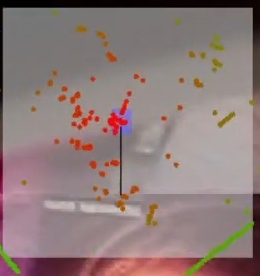
\includegraphics[width=0.8\textwidth]{./images/Pruebas/robot/MapaConRuidoSolar.png}
        \caption{Mapa con ruido por luz solar}
        \label{fig:MapaConRuidoLuzSolar}
    \end{figure}
% subsection An\'alisis tercera  (end)
    \subsection{Pruebas de aceptaci\'on en entornos complejos simulados y reales}
    Las pruebas de aceptaci\'on en entornos complejos se realizaron con el objetivo de verificar 
        que el sistema es capaz de operar bajo condiciones reales y simuladas, cumpliendo con 
        los requisitos funcionales establecidos para su despliegue en escenarios pr\'acticos. Una 
        de las pruebas clave fue la realizada durante el evento en el planetario del IPN, donde el 
        robot estuvo en funcionamiento durante dos horas en un entorno din\'amico y lleno de obst\'aculos, 
        lo que incluy\'o la presencia de ni\~nos en movimiento, muebles y luz solar directa.
    \vskip 0.5cm
    En esta prueba de aceptaci\'on, el robot fue sometido a un entorno complejo y real, lo que permiti\'o evaluar 
        su capacidad para reaccionar ante situaciones imprevistas y la efectividad de su sistema de navegaci\'on 
        aut\'onoma. A pesar de las interferencias causadas por la luz solar en el sensor LiDAR, el sistema logr\'o 
        operar de manera continua y sin fallos cr\'iticos. Sin embargo, se observaron limitaciones en la detecci\'on 
        de obst\'aculos en ciertas situaciones, como cuando los ni\~nos o los objetos estaban fuera del rango del 
        LiDAR o cuando la luz solar directa afectaba su precisi\'on.
    \vskip 0.5cm
    El entorno lleno de personas y la variabilidad de los objetos presentes proporcionaron una simulaci\'on adecuada 
        de escenarios reales en los que el robot podr\'ia operar. La prueba tambi\'en sirvi\'o para observar c\'omo el 
        sistema respond\'ia a la carga continua de funcionamiento prolongado. Aunque no se registraron fallos 
        significativos que impidieran el correcto funcionamiento del robot, el comportamiento observado 
        permiti\'o identificar \'areas de mejora, especialmente en cuanto a la detecci\'on de objetos porosos o 
        muy delgados, y la interferencia de se\~nales infrarrojas provenientes del sol.
    \vskip 0.5cm
    El proceso de aceptaci\'on fue validado por el profesor responsable, quien evalu\'o tanto el desempe\~no 
        del sistema en el entorno real como los datos obtenidos durante la prueba. Tras su an\'alisis, 
        el profesor concluy\'o que el robot cumpl\'ia con los criterios establecidos para su aceptaci\'on, 
        aunque con algunas recomendaciones para mejorar el rendimiento en condiciones extremas, como 
        las observadas en exteriores.
    \vskip 0.5cm
    La aprobaci\'on final del profesor, tras el an\'alisis de los resultados y la revisi\'on del desempe\~no en entornos 
        simulados y reales, confirma que el sistema est\'a listo para su implementaci\'on en otros escenarios 
        operativos m\'as complejos.
    \vskip 0.5cm
    A su vez como se menciona en la secci\'on \ref{sub:PruebasDeCarga02} se realiz\'o otra prueba de carga en la 
        Secretar\'ia de Hacienda y Cr\'edito P\'ublico, en la cual el robot estuvo en funcionamiento durante un 
        per\'iodo de 3 horas, con el objetivo de evaluar su capacidad para operar en un entorno din\'amico y lleno 
        de personas. Esta prueba proporcion\'o una valiosa evaluaci\'on del rendimiento del sistema en escenarios 
        extendidos y su capacidad para mantener la operaci\'on bajo condiciones diversas, lo que contribuye a la 
        validaci\'on general del sistema y su resistencia en situaciones prolongadas.
% subsection Pruebas de aceptaci\'on en entornos complejos simulados y reales (end)
    \subsection{Pruebas de carga y resistencia en escenarios extendidos para validaci\'on de fallos}
\label{sub:PruebasDeCarga02}
    Como parte de la validaci\'on del sistema en entornos complejos, se realiz\'o una prueba de carga  
        y resistencia durante un evento en el planetario del IPN. El robot estuvo en funcionamiento 
        continuo durante un per\'iodo de dos horas, con el objetivo de evaluar su capacidad para operar 
        en un entorno din\'amico y lleno de personas, incluidas condiciones espec\'ificas como la luz solar 
        directa y la presencia de m\'ultiples obst\'aculos m\'oviles, principalmente ni\~nos.
    \vskip 0.5cm
    Durante esta prueba, se observ\'o que el sistema mantuvo un rendimiento estable, a pesar de los desaf\'ios 
        que presentaba el entorno. Sin embargo, como se observ\'o en iteraciones anteriores, la luz del 
        sol interfer\'ia con la capacidad del sensor LiDAR para detectar correctamente los obst\'aculos, 
        lo cual se agravaba en \'areas donde los rayos solares incid\'ian directamente sobre los objetos. 
        Esto generaba inconsistencias en la detecci\'on de obst\'aculos, sobre todo cuando el robot interactuaba 
        con objetos en movimiento, como los ni\~nos que se encontraban en el lugar.
    \vskip 0.5cm
    Si bien no ocurrieron incidentes cr\'iticos durante las dos horas de funcionamiento, se grabaron aproximadamente 
        40 minutos de video como parte de la documentaci\'on del evento. Esta grabaci\'on incluye las interacciones 
        del robot con el entorno, permitiendo observar c\'omo el sistema respond\'ia a los desaf\'ios planteados, como 
        la presencia de ni\~nos y las variaciones en la luz natural. Aunque en gran parte del tiempo el robot oper\'o 
        de forma estable, estos eventos brindaron informaci\'on valiosa sobre las limitaciones del sistema en entornos reales.
    \vskip 0.5cm
    Puedes acceder al video de la prueba haciendo clic en el siguiente enlace: \url{https://drive.google.com/file/d/1p5S6dewukp-0Qsq_qk9K40o2LhSbtPgf/view?usp=drive_link}
    \vskip 0.5cm
    Esta prueba proporcion\'o una valiosa evaluaci\'on del rendimiento del sistema en escenarios extendidos y su 
        capacidad para mantener la operaci\'on bajo condiciones diversas, lo que contribuye a la validaci\'on general 
        del sistema y su resistencia en situaciones prolongadas.
    \vskip 0.5cm
    A su vez, se hizo otra prueba de carga en la Secretar\'ia de Hacienda y Cr\'edito P\'ublico, en la cual el robot 
        estuvo en funcionamiento durante un per\'iodo de 3 horas, con el objetivo de evaluar su capacidad para operar 
        en un entorno din\'amico y lleno de personas. Se puede observar aqu\'i: \url{https://drive.google.com/file/d/1p5S6dewukp-0Qsq_qk9K40o2LhSbtPgf/view?usp=drive_link}
% subsection Pruebas de carga y resistencia en escenarios extendidos para validaci\'on de fallos (end)
    \subsection{Evaluaci\'on de tercera iteraci\'on del desempe\~no del robot de pruebas integrales}

% Tabla de evaluaci\'on de la primera iteraci\'on
\begin{table}[htbp]
    \centering
    \caption{Evaluaci\'on de la tercera iteraci\'on del desempe\~no del robot de pruebas integrales}
    \label{tab:EvaluacionPrimeraIteracion}
    \resizebox{\textwidth}{!}{%
    \begin{tabular}{|c|c|c|c|}
    \hline
    \rowcolor[HTML]{C0C0C0} 
    \textbf{Criterio} & \textbf{Descripci\'on} & \textbf{Puntuaci\'on (1-5)} & \textbf{Observaciones} \\ \hline
    \textbf{Precisi\'on de Detecci\'on del LiDAR} & Evaluar la capacidad del LiDAR para detectar obst\'aculos a diversas distancias, especialmente en rangos cortos (<10 cm). & 4 & Perfeccionado, sin embargo hay espacio de mejora \\ \hline
    \textbf{Estabilidad del Hardware (Motores y Controlador)} & Evaluar si los motores y el controlador operan de manera estable, sin sobrecalentamientos o fallos. & 4 & No Aplica \\ \hline
    \textbf{Navegaci\'on Aut\'onoma} & Evaluar la capacidad del robot para moverse de manera aut\'onoma y evitar obst\'aculos en un entorno controlado. & 4 & Es mucho mejor que antes, sobre todo ahora puede pasar por lugares estrechos \\ \hline
    \textbf{Reacci\'on a Obst\'aculos Peque\~nos/Din\'amicos} & Evaluar la rapidez y precisi\'on con que el robot detecta y responde a obst\'aculos peque\~nos o en movimiento. & 4.5 & Los rangos fueron calculados a la medida \\ \hline
    \textbf{Resistencia al Funcionamiento Prolongado} & Evaluar si el robot puede operar de manera continua sin fallos durante largos per\'iodos de tiempo (pruebas de carga). & 3 & No hay presupuesto para cargador \\ \hline
    \textbf{Sincronizaci\'on de Sensores} & Evaluar la capacidad del sistema para sincronizar correctamente los datos del LiDAR y las c\'amaras (formato YUV/RGB). & 4 & No aplica \\ \hline
    \textbf{Capacidad de Esquivar Obst\'aculos} & Evaluar si el robot puede evitar colisiones con precisi\'on, bas\'andose en los datos del LiDAR. & 3.5 & Dura aproximadamente 2 horas y media encendido. \\ \hline
    \textbf{Consumo Energ\'etico} & Evaluar la eficiencia energ\'etica del sistema durante el funcionamiento prolongado. & 4 & No Aplica \\ \hline
    \end{tabular}%
    }
\end{table}